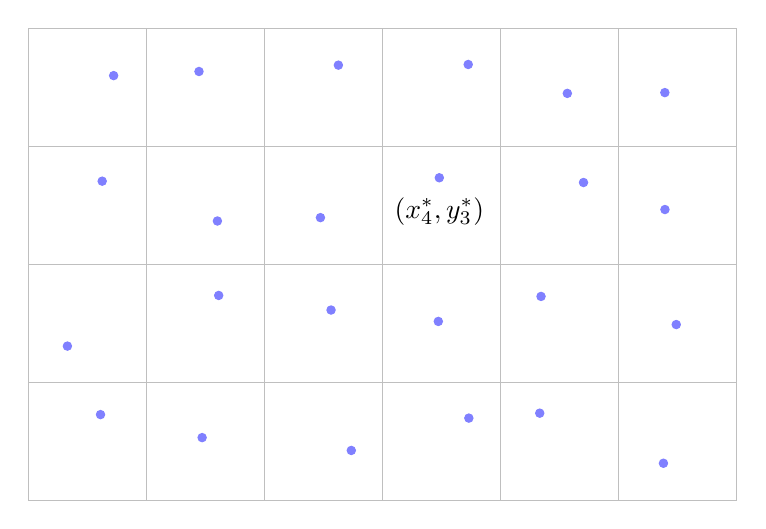
\begin{tikzpicture}[scale=1.5]
    \draw[step=1,draw=gray!50] (0,0) grid (6,4);
    \foreach \i in {1,...,6}{
        \foreach \j in {1,...,4}{
            \pgfmathparse{rnd}
            \pgfmathsetmacro{\x}{\i - 0.25 - \pgfmathresult/2.2}
            \pgfmathparse{rnd}
            \pgfmathsetmacro{\y}{\j - 0.25 - \pgfmathresult/2.2}
            \filldraw[blue!50] (\x,\y) circle (1pt);
            \ifnum\i=4
                \ifnum\j=3
                    \node[label={[black]270:$(x_{\i}^*,y_{\j}^*)$}] at (\x,\y) {};
                \fi
            \fi
        }
    }
\end{tikzpicture}
    